\documentclass[twocolumn, 10.5pt,a4j]{ltjsarticle}

% 卒業研究報告書スタイルファイル
\usepackage{twocolums}

\usepackage[tocgraduated]{tocstyle}
% ソースコード表示
\usepackage{listings}
% 色
\usepackage{xcolor}
% 数学関連
\usepackage{amsmath, amssymb}
% リスト制御
\usepackage{enumitem}
% 画像
\usepackage{graphicx}
% shaded環境の背景色の定義
\definecolor{shadecolor}{gray}{0.80}
% 枠
\usepackage{ascmac}
\usepackage{tcolorbox}
% url表記
\usepackage{url}
% ハイパーリンク
\usepackage[pdfencoding=auto]{hyperref}
% フォント
\usepackage{layouts/lualatexsets/fonts}
% Tikz関係
\usepackage{tikz}
% 証明などのスタイル
\usepackage{layouts/others/theorem}
% セクションの表示スタイル
%\usepackage{layouts/others/section}
% ベクトル表記
\usepackage{bm}
\def\vector#1{\boldsymbol{#1}}
% 疑似コード
% \usepackage{algorithm}
% \usepackage{algorithmic}
% 画像・図表等のrefコマンド
\def\thmref#1{Thm. \ref{#1}}
\def\lmmref#1{Lemma. \ref{#1}}
\def\figref#1{図\ref{#1}}
\def\eqref#1{(\ref{#1})式}
\def\tableref#1{表\ref{#1}}

%%% ドキュメント情報 %%%
% 著者
\author{萩原 涼介}
% タイトル
\title{クラスタ数推定に用いる最適な情報量基準の探求}
% 指導教員
\adviser{藤田 一寿}
% 発表番号
\presentationnumber{A-07}

\begin{document}
\maketitle

\section{はじめに}

クラスタリングとはデータを教師なし学習により任意の数のクラスタに分ける手法である.
$k$-means を始めとする多くのクラスタリング手法では,予めクラスタ数がわかっているものとして,
クラスタ数を指定しクラスタリングを行う.しかし,データに対し最適なクラスタ数を指定しなければ,最適なクラスタリング結果を得ることはできない.
しかし,一般にクラスタ数が事前にわかっていない.その為,クラスタ数を推定することは重要な課題となっている.
クラスタ数推定を行う際,よく用いられるのが情報量規準と呼ばれれる指標である.
情報量規準とは簡単に言えば確率分布とデータの分布の当てはまり具合を表すものである.
その情報量基準は多くの研究者により様々なものが提案されている.
しかし,どの情報量規準がどのようなデータに対し有効かは分かっていない.
そこで本研究では,クラスタ数推定に用いる情報量規準として最適なものを数値実験を通し明らかにする.

\section{実験手法}
本研究ではX-meansと呼ばれる手法を用い,クラスタ数推定およびクラスタリングを行った.
X-meansは情報量基準を用い,クラスタ数を決定する.
前期は,AIC, cAIC, BICと呼ばれる3つの情報量規準をそれぞれ用いクラスタ数推定およびククラスタリングを行い,その結果の比較を行った.
精度の評価には,正規化相互情報量 (NMI) および Purityを用いた.
それぞれの指標は1に近づくほど良いクラスタリング結果であると言える.

\section{実験結果}
数値実験では\figurenum{fig:2dim}のような分散$\sigma^2 = 1$の2次元混合等方Gauss分布をデータセットとして用いた.
このデータセットは5つの等方Gauss分布で構成される.そして各クラスタは500個のデータ点を持つ.
このデータセットに対し,AIC, cAIC, AIC, 対数尤度関数を情報量規準としてそれぞれ採用したX-meansによるクラスタリングを行った.

\tableref{table:2dim}は推定したクラスタ数とクラスタリングの精度を表す.それぞれの数値は100回実行した結果を平均したものである.
この結果,混合等方Gauss分布ではBICとcAICが適していることがわかった.
AICを採用した場合,平均値はよいが,クラスタ数を過大に見積もってしまう問題が生じた.

\begin{figure}[htbp]
  \begin{center}
    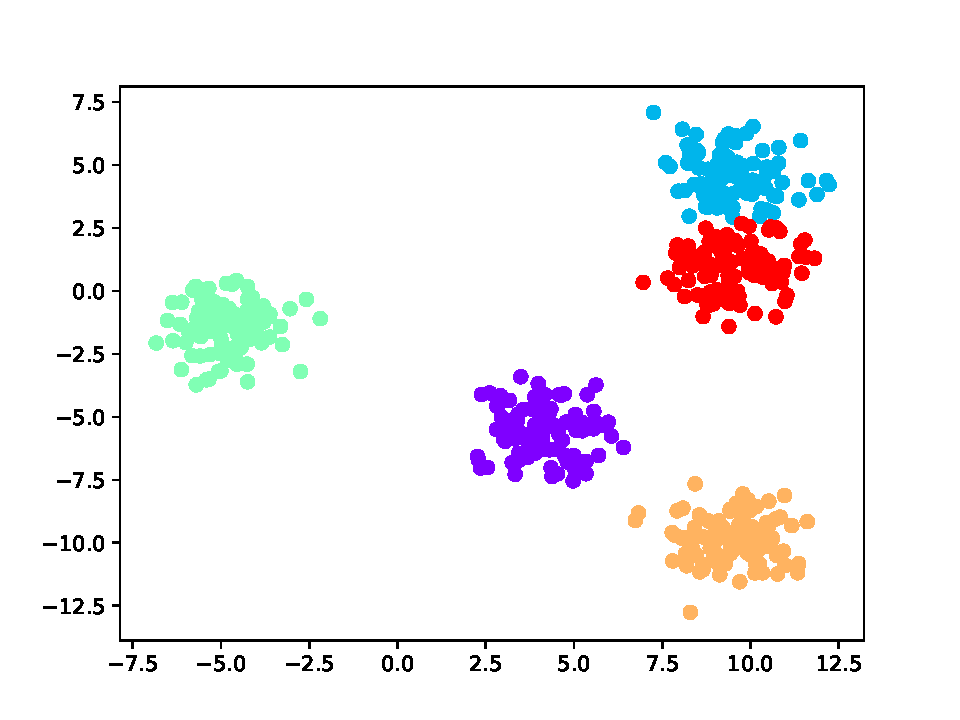
\includegraphics[width=1.0\linewidth]{./img/BIC_2.pdf}
      \caption{2次元空間のクラスタリング例}
      \label{fig:2dim}
  \end{center}
\end{figure}
\begin{table}[htb]
  \centering
  \caption{2次元空間におけるクラスタリング結果}
  \label{table:2dim}
  \begin{tabular}{|c|c|c|c|} \hline
    分割停止規準 & クラスタ数 & NMI & Purity \\\hline
    BIC  & 4.58 & 0.88281 & 0.84459\\
    cAIC & 4.55 & 0.89993 & 0.85329\\
    AIC  & 4.69 & 0.88147 & 0.83642\\
    対数尤度関数 & 5.32 & 0.91572 & 0.85700\\\hline
  \end{tabular}
\end{table}

\section{おわりに}
今後は他の情報量規準を用いたクラスタリングや,クラスタリング対象のデータを変更するなどして,
それぞれのデータのクラスタリングに最も適した情報量規準を探求していきたい.

\vspace{1em}
\noindent【研究目標】\\
クラスタ数推定に用いる最適な情報量規準を探求する

\vspace{1em}
\noindent【課題項目】\\
$\bigcirc$: 文献調査, $\bigcirc$: クラスタリングの実装, $\bigtriangleup$: 数値実験\noindent
\end{document}
